%!TEX root = ../../report.tex

\begin{figure}[H]
	\newcommand{\figurewidth}{0.3\textwidth}
	\begin{subfigure}[b]{\figurewidth}
        \centering
        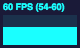
\includegraphics{images/testing/fps}
        \caption{FPS tool for measuring frames rendered in the last second.}
        \label{fig:fps_tool}
    \end{subfigure}
    \begin{subfigure}[b]{\figurewidth}
        \centering
    	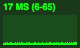
\includegraphics{images/testing/ms}
        \caption{MS tool for measuring milliseconds to render a frame.}
        \label{fig:ms_tool}
    \end{subfigure}
    \begin{subfigure}[b]{\figurewidth}
        \centering
        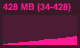
\includegraphics{images/testing/mb}
        \caption{MB tool for measuring the size of allocated memory.}
        \label{fig:mb_tool}
    \end{subfigure}
	\caption{JavaScript Performance Monitor.}
	\label{fig:js_performance_monitor}
\end{figure}
